\documentclass[a4paper,12pt]{article}
\usepackage{amssymb} % needed for math
\usepackage{amsmath} % needed for math
\usepackage[utf8]{inputenc} % this is needed for german umlauts
\usepackage[ngerman]{babel} % this is needed for german umlauts
\usepackage[T1]{fontenc}    % this is needed for correct output of umlauts in pdf
\usepackage[margin=2.5cm]{geometry} %layout
\usepackage{booktabs}

% this is needed for forms and links within the text
\usepackage{hyperref}  

% glossar, see http://en.wikibooks.org/wiki/LaTeX/Glossary
% has to be loaded AFTER hyperref so that entries are clickable
\usepackage[nonumberlist]{glossaries} 

% The following is needed in order to make the code compatible
% with both latex/dvips and pdflatex.
\ifx\pdftexversion\undefined
\usepackage[dvips]{graphicx}
\else
\usepackage[pdftex]{graphicx}
\DeclareGraphicsRule{*}{mps}{*}{}
\fi

\makeglossary 

%%%%%%%%%%%%%%%%%%%%%%%%%%%%%%%%%%%%%%%%%%%%%%%%%%%%%%%%%%%%%%%%%%%%%%
% Variablen                                 						 %
%%%%%%%%%%%%%%%%%%%%%%%%%%%%%%%%%%%%%%%%%%%%%%%%%%%%%%%%%%%%%%%%%%%%%%
\newcommand{\authorName}{Dustin Spallek, Rene Kretschmer, Christof Rode, Jana Wengenroth, Malte Scheller, Daniel Schruhl}
\newcommand{\projektName}{Microservices mit Angular}
\newcommand{\tags}{\authorName, Lastenheft}
\newcommand{\glossarName}{Glossar}
\title{\projektName~(Pflichtenheft)}
\author{\authorName}
\date{\today}

%%%%%%%%%%%%%%%%%%%%%%%%%%%%%%%%%%%%%%%%%%%%%%%%%%%%%%%%%%%%%%%%%%%%%%
% PDF Meta information                                 				 %
%%%%%%%%%%%%%%%%%%%%%%%%%%%%%%%%%%%%%%%%%%%%%%%%%%%%%%%%%%%%%%%%%%%%%%
\hypersetup{
  pdfauthor   = {\authorName},
  pdfkeywords = {\tags},
  pdftitle    = {\projektName~(Pflichtenheft)}
} 
 
%%%%%%%%%%%%%%%%%%%%%%%%%%%%%%%%%%%%%%%%%%%%%%%%%%%%%%%%%%%%%%%%%%%%%%
% Create a shorter version for tables. DO NOT CHANGE               	 %
%%%%%%%%%%%%%%%%%%%%%%%%%%%%%%%%%%%%%%%%%%%%%%%%%%%%%%%%%%%%%%%%%%%%%%
\newcommand\addrow[2]{#1 &#2\\ }

\newcommand\addheading[2]{#1 &#2\\ \hline}
\newcommand\tabularhead{\begin{tabular}{lp{13cm}}
\hline
}

\newcommand\addmulrow[2]{ \begin{minipage}[t][][t]{2.5cm}#1\end{minipage}% 
   &\begin{minipage}[t][][t]{8cm}
    \begin{enumerate} #2   \end{enumerate}
    \end{minipage}\\ }

\newenvironment{usecase}{\tabularhead}
{\hline\end{tabular}}




%%%%%%%%%%%%%%%%%%%%%%%%%%%%%%%%%%%%%%%%%%%%%%%%%%%%%%%%%%%%%%%%%%%%%%
% THE DOCUMENT BEGINS             	                              	 %
%%%%%%%%%%%%%%%%%%%%%%%%%%%%%%%%%%%%%%%%%%%%%%%%%%%%%%%%%%%%%%%%%%%%%%
\begin{document}
 \pagenumbering{roman}
 \begin{titlepage}
\maketitle
\thispagestyle{empty} % no page number

\begin{verbatim}












\end{verbatim}


  \begin{tabular}[t]{ll}
	Projekt:       & \quad \projektName \\[1.2ex]
  \end{tabular}

\begin{tabularx}{\textwidth}{|l|l|X|}
\hline
\textbf{Version} & \textbf{Datum} & \textbf{Autor(en)} \\
\hline
\hline
1.0 & 19.09.2016 & \authorName \\
2.0 & 10.10.2016 & \authorName \\
\hline
\end{tabularx}
\end{titlepage}
         % Deckblatt.tex laden und einfügen
 \setcounter{page}{2}
 \tableofcontents          % Inhaltsverzeichnis ausgeben
 \clearpage
 \pagenumbering{arabic}
 
\section{Zielbestimmung}
\subsection{Musskriterien}
%%%%%%%%%%%%%%%%%%%%%%%%%%%%%%%%%%%%%%%%%%%%%%%%%%%%%%%%%%%%%%%%%%%%%%
% Was muss das Programm können?                   					 %
%%%%%%%%%%%%%%%%%%%%%%%%%%%%%%%%%%%%%%%%%%%%%%%%%%%%%%%%%%%%%%%%%%%%%%
\begin{usecase}
  \addheading{Nummer}{Beschreibung} 
  \addrow{/FA10/}{Lorem ipsum dolor sit amet, consetetur sadipscing elitr, sed diam}
  \addrow{/FA20/}{Lorem ipsum dolor sit amet, consetetur sadipscing elitr}
  \addrow{/FA30/}{adasdfasdf asdf asdfas}
\end{usecase}

\subsection{Wunschkriterien}
%%%%%%%%%%%%%%%%%%%%%%%%%%%%%%%%%%%%%%%%%%%%%%%%%%%%%%%%%%%%%%%%%%%%%%
% Was muss das Programm können?                   					 %
%%%%%%%%%%%%%%%%%%%%%%%%%%%%%%%%%%%%%%%%%%%%%%%%%%%%%%%%%%%%%%%%%%%%%%
\begin{usecase}
  \addheading{Nummer}{Beschreibung} 
  \addrow{/FA10/}{Lorem ipsum dolor sit amet, consetetur sadipscing elitr, sed diam}
  \addrow{/FA20/}{Lorem ipsum dolor sit amet, consetetur sadipscing elitr}
  \addrow{/FA30/}{adasdfasdf asdf asdfas}
\end{usecase}

\subsection{Abgrenzungskriterien}
%%%%%%%%%%%%%%%%%%%%%%%%%%%%%%%%%%%%%%%%%%%%%%%%%%%%%%%%%%%%%%%%%%%%%%
% Was muss das Programm können?                   					 %
%%%%%%%%%%%%%%%%%%%%%%%%%%%%%%%%%%%%%%%%%%%%%%%%%%%%%%%%%%%%%%%%%%%%%%
\begin{usecase}
  \addheading{Nummer}{Beschreibung} 
  \addrow{/FA10/}{Lorem ipsum dolor sit amet, consetetur sadipscing elitr, sed diam}
  \addrow{/FA20/}{Lorem ipsum dolor sit amet, consetetur sadipscing elitr}
  \addrow{/FA30/}{adasdfasdf asdf asdfas}
\end{usecase}


\section{Produkteinsatz}
%%%%%%%%%%%%%%%%%%%%%%%%%%%%%%%%%%%%%%%%%%%%%%%%%%%%%%%%%%%%%%%%%%%%%%
% Wer ist die Zielgruppe?                   						 %
%%%%%%%%%%%%%%%%%%%%%%%%%%%%%%%%%%%%%%%%%%%%%%%%%%%%%%%%%%%%%%%%%%%%%%
Der Microservice soll in die Infrastruktur von Symphony eingegliedert werden, um für Anbieter die Funktion der Anreicherung ihrer Produktdaten zu ermöglichen.

\subsection{Zielgruppe}
Unsere Zielgruppe sind alle Mitarbeiter der Anbieter, die einen Zugang zum System haben.

\subsection{Anwendungsbereiche}
Administrative Anwendungsbereiche zur Verwaltung und Anreicherung der Anbieter und Produktdaten.

\section{Funktionale Anforderungen}
%%%%%%%%%%%%%%%%%%%%%%%%%%%%%%%%%%%%%%%%%%%%%%%%%%%%%%%%%%%%%%%%%%%%%%
% Was muss das Programm können?                   					 %
%%%%%%%%%%%%%%%%%%%%%%%%%%%%%%%%%%%%%%%%%%%%%%%%%%%%%%%%%%%%%%%%%%%%%%
\begin{usecase}
  \addheading{Nummer}{Beschreibung} 
  \addrow{/FA10/}{Lorem ipsum dolor sit amet, consetetur sadipscing elitr, sed diam}
  \addrow{/FA20/}{Lorem ipsum dolor sit amet, consetetur sadipscing elitr}
  \addrow{/FA30/}{adasdfasdf asdf asdfas}
\end{usecase}

\section{Produktdaten}
%%%%%%%%%%%%%%%%%%%%%%%%%%%%%%%%%%%%%%%%%%%%%%%%%%%%%%%%%%%%%%%%%%%%%%
% Auf welchen Daten arbeitet das Produkt?                            %
%%%%%%%%%%%%%%%%%%%%%%%%%%%%%%%%%%%%%%%%%%%%%%%%%%%%%%%%%%%%%%%%%%%%%%
\begin{usecase}
  \addheading{Nummer}{Beschreibung} 
  \addrow{/PD10/}{Produkte haben einen Namen}
  \addrow{/PD20/}{Produkte haben eine Kurzbeschreibung}
  \addrow{/PD30/}{Produkte haben eine Detailbeschreibung}
  \addrow{/PD40/}{Produkte haben eine Feature Tabelle}
  \addrow{/PD50/}{Ein Produkt hat ein Hauptbild}
  \addrow{/PD60/}{Ein Produkt hat Medien in einer Galerie} 
  \addrow{/PD70/}{Anbieter haben mehrere Produkte}
  \addrow{/PD80/}{Anbieter haben einen Namen}
  \addrow{/PD90/}{Anbieter haben eine Kurzbeschreibung}
  \addrow{/PD100/}{Anbieter haben eine Detailbeschreibung}
  \addrow{/PD110/}{Anbieter haben eine Feature Tabelle}
  \addrow{/PD120/}{Ein Anbieter hat ein Hauptbild}
  \addrow{/PD130/}{Ein Anbieter hat Medien in einer Galerie} 
  \addrow{/PD140/}{Ein Feature in der Feature Tabelle hat einen Titel und eine Beschreibung}
  \addrow{/PD150/}{Eine Feature Tabelle hat mehrere Features}
  \addrow{/PD160/}{Medien in der Galerie können PDFs oder Bilder sein}
  \addrow{/PD170/}{Ein User hat einen Namen und ein Passwort}
\end{usecase}

\section{Nichtfunktionale Anforderungen}
\begin{usecase}
  \addheading{Nummer}{Beschreibung} 
  \addrow{/NF10/}{asdf asdf asdf asdf asdf asdf }
  \addrow{/NF20/}{ asdf asdf asdftergfgasdgewr asdfh}
\end{usecase}

\clearpage

\section{Systemmodelle}

\subsection{Datenmodell}

\begin{figure}[!htb]
  \centering
     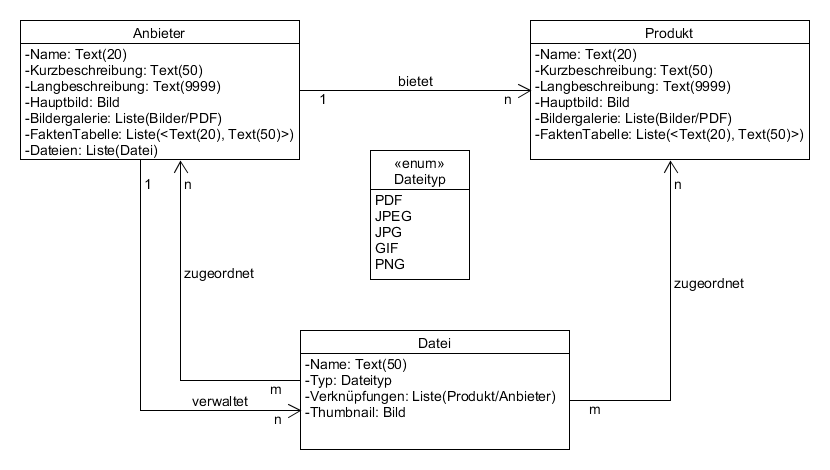
\includegraphics[width=1.0\textwidth]{FDM.png}
  \caption{Fachliches Datenmodell}
  \label{fig:fmd}
\end{figure}

\clearpage

\subsection{Benutzeroberfläche}

\begin{figure}[!htb]
  \centering
     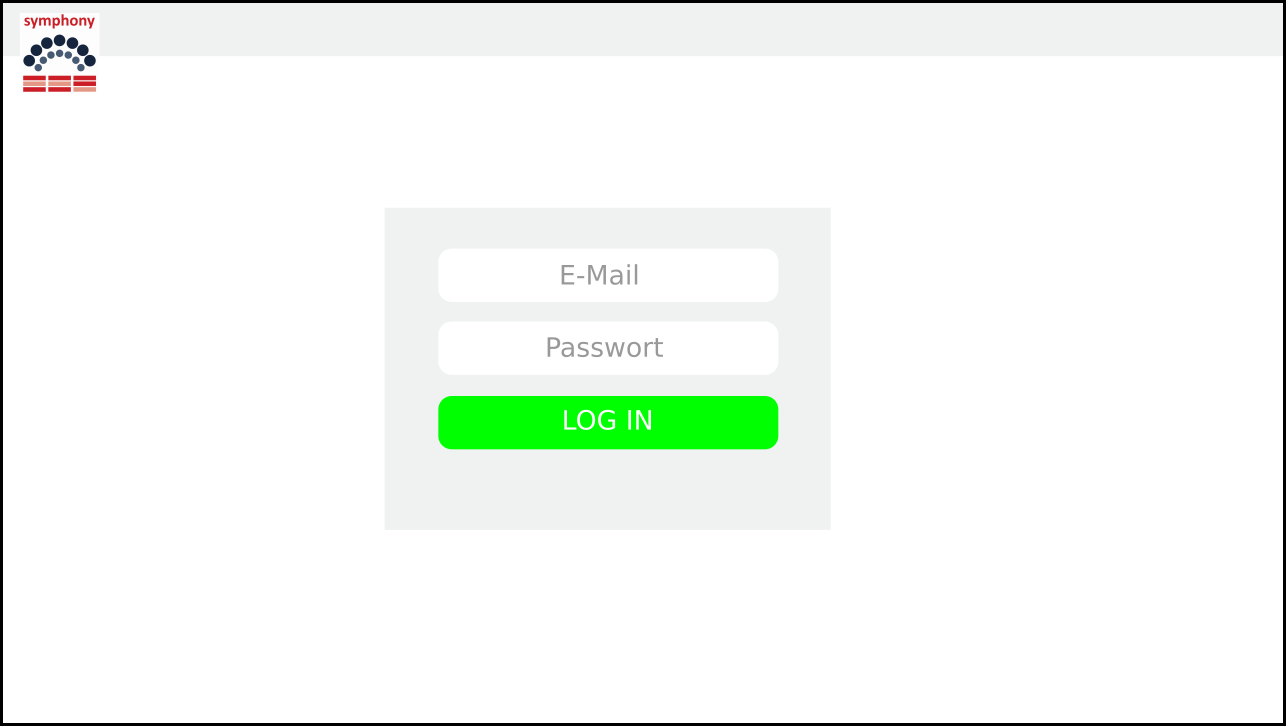
\includegraphics[width=1.0\textwidth]{projmicro_login.png}
  \caption{Login Mockup}
  \label{fig:login}
\end{figure}

\begin{figure}[!htb]
  \centering
     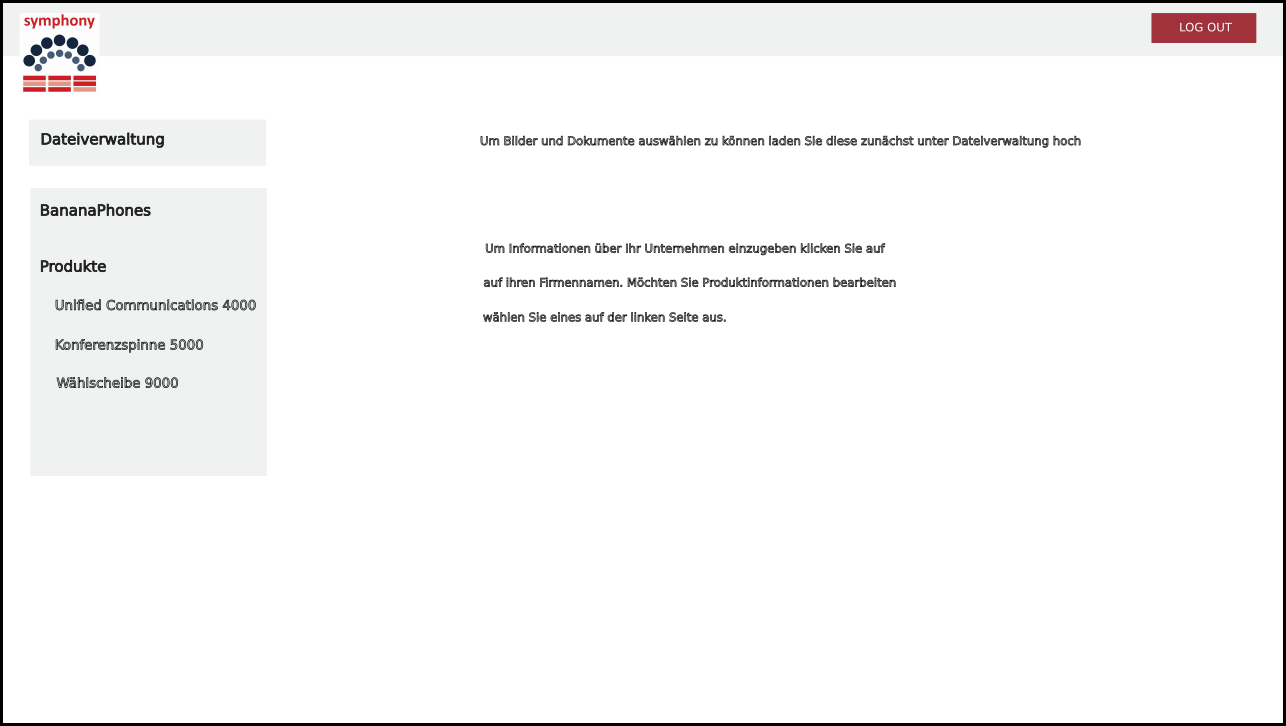
\includegraphics[width=1.0\textwidth]{projmicro_auswahl.png}
  \caption{Auswahlfenster Mockup}
  \label{fig:selection}
\end{figure}

\begin{figure}[!htb]
  \centering
     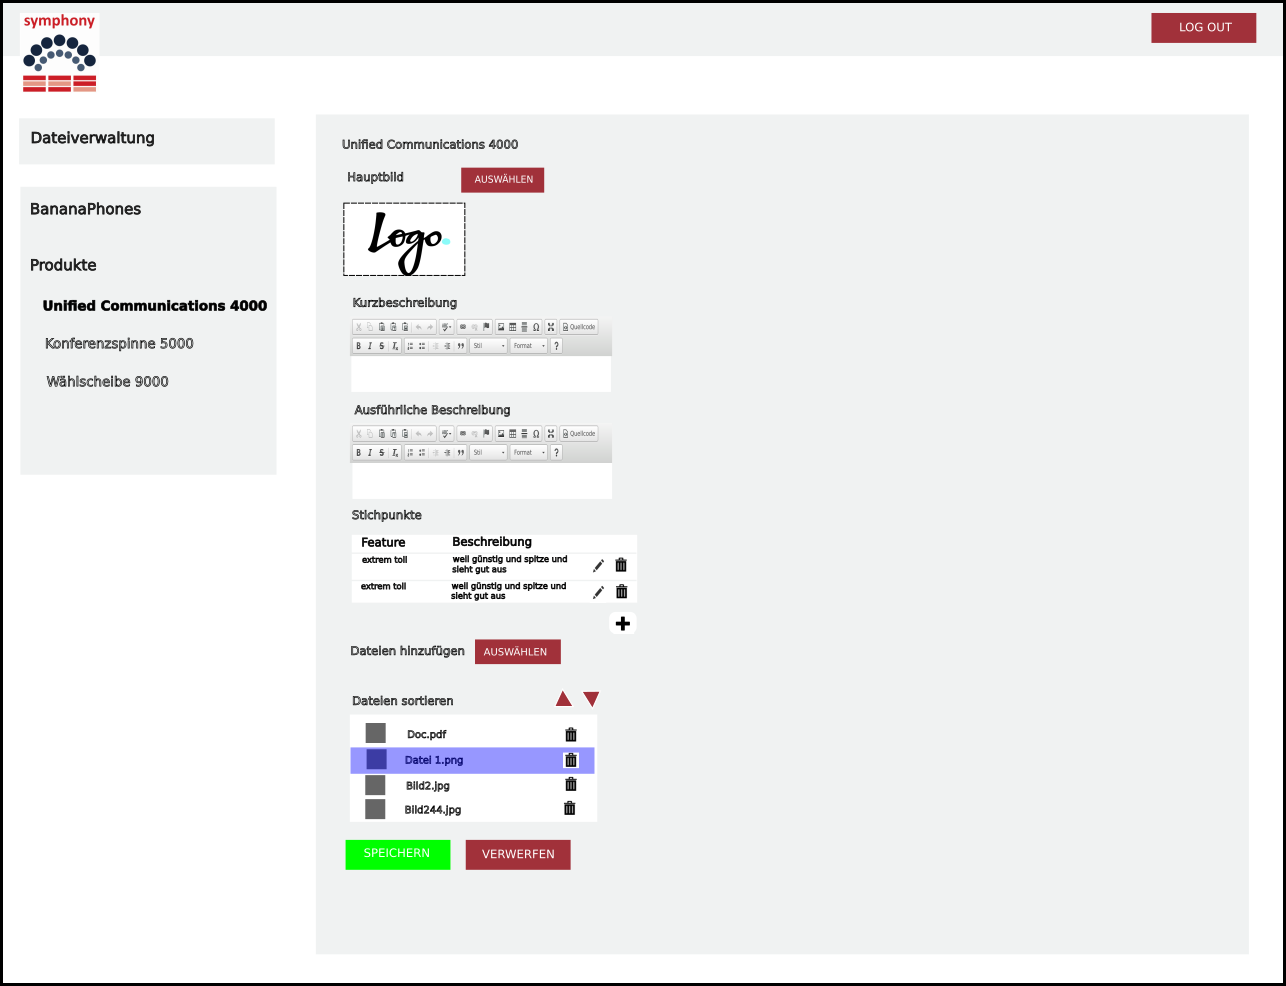
\includegraphics[width=1.0\textwidth]{projmicro_edit.png}
  \caption{Datensatz Bearbeitungs Mockup}
  \label{fig:edit}
\end{figure}

\begin{figure}[!htb]
  \centering
     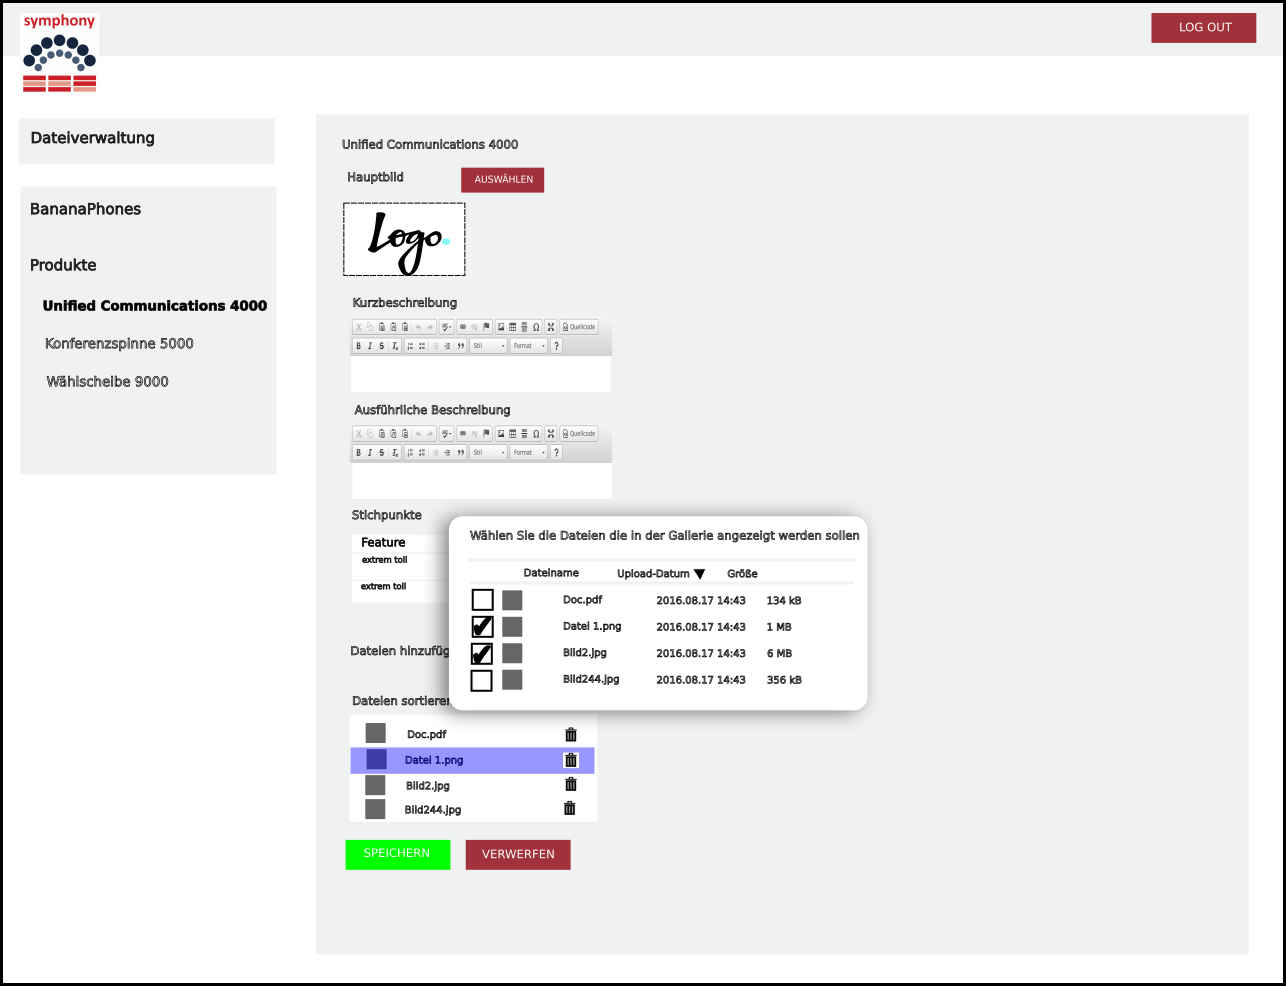
\includegraphics[width=1.0\textwidth]{projmicro_edit_dateiauswahl.png}
  \caption{Datensazu Bearbeitungs Mockup mit Upload}
  \label{fig:edit_file}
\end{figure}

\begin{figure}[!htb]
  \centering
     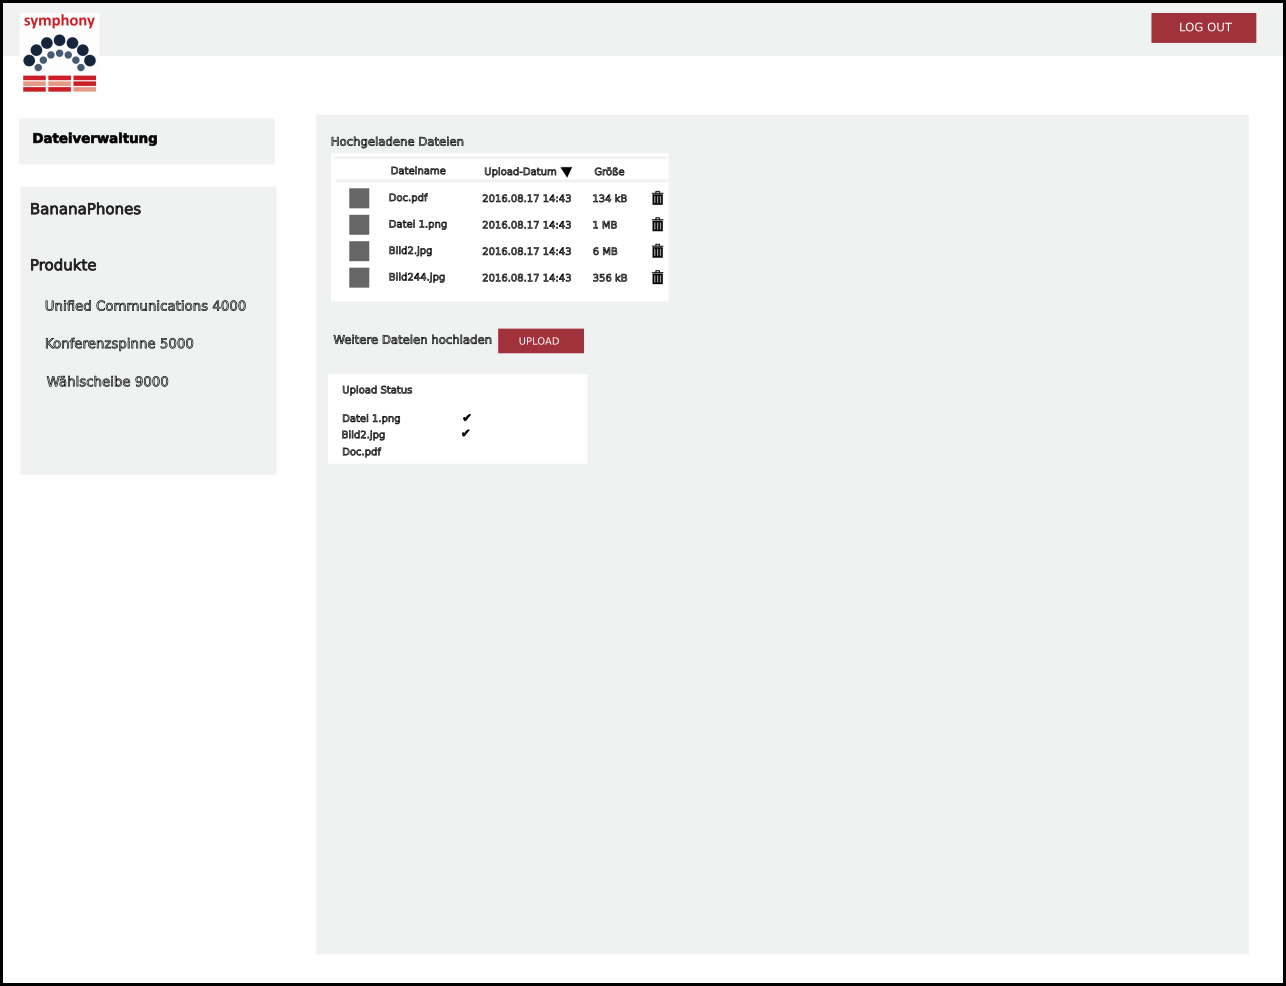
\includegraphics[width=1.0\textwidth]{projmicro_upload.png}
  \caption{Dateiverwaltung Mockup}
  \label{fig:selection}
\end{figure}

\end{document}
